% !TEX program = xelatex
% !BIB program = biber

\documentclass[11pt]{article}

\usepackage{biblatex}
\usepackage{listings}
\usepackage{xcolor}
\usepackage{fontspec}
\usepackage{graphicx}
\usepackage{amsmath}
\usepackage{amssymb}
\usepackage{float}
\usepackage{caption}
\usepackage{pdfpages}

\setmonofont[Contextuals={Alternate}, Scale=0.8]{Fira Code}

\addbibresource{viper.bib}
\addbibresource{silicon.bib}
\addbibresource{patterns.bib}
\addbibresource{intellij.bib}
\addbibresource{caffeine.bib}
\addbibresource{smallfoot.bib}
\addbibresource{macros.bib}
\addbibresource{vercors.bib}
\addbibresource{nagini.bib}
\addbibresource{gobra.bib}
\addbibresource{prusti.bib}
\addbibresource{vyper.bib}
\addbibresource{z3.bib}

\parskip=1em
\parindent=0pt

\definecolor{codegrey}{rgb}{0.9,0.9,0.9}
\definecolor{commentgrey}{rgb}{0.5,0.5,0.5}

\lstdefinestyle{mystyle}{
    basicstyle=\ttfamily,
    keywordstyle=\bfseries,
    commentstyle=\color{commentgrey},
    %backgroundcolor=\color{codegrey},
    frame=single,
    numbers=left,
}
\lstset{style=mystyle}

\DeclareMathOperator{\perm}{\mathbin{\#}}

\begin{document}

    \pagenumbering{gobble}
    \begin{titlepage}
        \begin{center}
            \textit{Bachelor's Thesis}\\
            \vspace{0.5cm}
            \textbf{\Huge Performance Improvements of a Program Verifier}\\
            \vfill   
            Fabian Bösiger\\
            Supervised by Dr. Malte Schwerhoff\\
            \vspace{0.2cm}
            Programming Methodology Group\\
            Department of Computer Science\\
            ETH Zürich\\
            \vspace{0.2cm}
            \today
        \end{center}
    \end{titlepage}
    \newpage

    \begin{abstract}
        \parskip=1em
        \parindent=0pt
        \noindent

        To advance program verification in practice,
        fast verification is crucial as it provides a more streamlined experience for developers.
        This thesis explores two different approaches to improve performance of
        the Silicon program verification backend for the Viper
        verification infrastructure.

        In the first part,
        we explore the concept of applying the flyweight pattern on Silicon's AST structures.
        Applying the flyweight pattern avoids multiple instances of structurally equal AST nodes
        existing at the same time. This allows us to replace structural and recursive
        equality checks with reference equality checks, with the goal of improving performance of equality checks.

        In the second part, we introduce more sophisticated ways to join symbolic execution paths in
        Silicon, after having branched on conditional expressions, implications and if-statements.
    \end{abstract}
    \newpage

    \renewcommand{\abstractname}{Acknowledgements}
    \begin{abstract}
        \parskip=1em
        \parindent=0pt
        \noindent

        I would like to thank my supervisor, Malte Schwerhoff, who provided
        me with the opportunity to write this thesis. The time
        and effort he expended to help and advice me was highly appreciated.

        Furthermore, I'd like to thank Peter Müller and his group for sparking interest and providing insight
        into topics such as these.

        Last but not least, I'd like to express my gratitude towards my family for providing
        me with a very pleasant home office environment.
    \end{abstract}
    \newpage

    \setcounter{tocdepth}{2}
    \tableofcontents
    \newpage

    \pagenumbering{arabic}

    \section{Introduction}

    Viper \cite{viper} is a verification infrastructure on top of which verification tools
    for different programming languages can be built. Silicon \cite{silicon} is a backend for Viper,
    which is based on Smallfoot-style \cite{smallfoot} symbolic execution. 
    To advance program verification in practice,
    fast verification is crucial as it provides a more streamlined experience for developers.
    This is the reason why one of Silicon's stated goals is performance:

    \begin{quote} 
        ``The verifier should enable an IDE-like experience: it should be
        sufficiently fast such that users can continuously work on verifying
        programs [...]'' \cite{silicon}
    \end{quote}

    In this thesis, we explore two different approaches to improving performance of Silicon.

    \subsection*{First Approach}

    Silicon internally uses abstract syntax trees (AST) to represent
    the structure of a program as a tree data structure. As with any other tree structure,
    ASTs can be traversed, searched, transformed and so forth. During such operations,
    subtrees within the AST are potentially checked for equality many times.  Moreover, equality checks
    also occur in operations on collections of AST subtrees, for example in finding
    a specific subtree, which may add additional performance overhead.

    Equality checks can't easily be avoided, but they can be implemented in a more performant way.
    Silicon's AST nodes are called terms, which represent different program operations.
    \texttt{Plus(IntLiteral(1), IntLiteral(2))} represents the program code $1 + 2$. \texttt{Plus}, \texttt{IntLiteral(1)}
    and \texttt{IntLiteral(2)} are called terms.
    Currently in Silicon, new term instances are created independently of already existing ones, which potentially leads 
    to the coexistence of multiple structurally equal term instances. Subterm equality is checked in a
    structural and recursive manner. In part \ref{part-1} of working towards a potential improvement in performance,
    we explore the concept of applying the flyweight pattern \cite{patterns} on AST terms to only ever have
    one instance of some term structure, thus avoiding the need for structural and recursive equality checks.

    \subsection*{Second Approach}

    For verifying a program, Silicon uses the symbolic execution approach, where the program is interpreted,
    and a symbolic state keeps track of all possible program states at the current point of execution, for all
    possible input values of the program. When encountering certain expressions or statements, for example an
    if-statement, symbolic execution branches with the assumptions of the corresponding program path.

    Silicon currently only joins these branches for some simple cases. In other cases,
    branches aren't joined, which results in all statements later down the verification path
    being evaluated essentially twice, but with different assumptions in each branch. Both of these
    verification paths may branch again, potentially leading to exponential growth in the number of branches.
    In an effort to improve performance, part \ref{part-2} of this thesis focuses on implementing 
    joining of execution paths or more complex cases, which ultimately leads to fewer active branches.

    \part{Flyweight ASTs;\newline A Study in Applied Laziness} \label{part-1}
    \begin{center}
        \vspace{3cm}
        
\includegraphics[width=0.7\textwidth]{fly}
    \end{center}

    \newpage
    \section{Approach}

    In the following sections we discuss our approach of implementing the flyweight pattern on
    ASTs, and the advantage of using code generation via metaprogramming for our implementation.

    \subsection{Implementation of Flyweight ASTs}

    Currently in Silicon, new term instances are created independently of already existing ones, which potentially leads 
    to the coexistence of multiple structurally equal term instances. Subterm equality is checked in a
    structural and recursive manner.
    However the AST used in Silicon is immutable, so the flyweight pattern \cite{patterns}
    can be applied on AST terms.
    To do this, a pool of term instances is maintained. Whenever a term
    is to be created, the components of this new term is compared with the
    pool of existing terms. If a term with the same components already exists,
    a reference to the existing term is returned and
    the creation of a new instance is avoided. Otherwise, a new term is created and added to
    the pool.

    This gives the guarantee that there are no two instances of the
    same term in our pool, meaning every two structurally equal terms point to the same
    underlying object in memory. Comparing terms for structural equality then boils
    down to a cheap reference equality check, and recursive equality checks can be avoided,
    at the cost of increased overhead at the creation of a term instance due to the flyweight pattern.

    \begin{figure}[H]
        \begin{center}
            \begin{minipage}{.4\textwidth}
                \begin{center}
                    \includegraphics[width=1.0\textwidth]{no-flyweight.png}
                    \caption{Example AST without using the flyweight pattern. Multiple structurally equal instances of the some subterm may exist in the AST.}
                    \label{fig:no-flyweight-ast}
                \end{center}
            \end{minipage}
            \hspace{.1\textwidth}
            \begin{minipage}{.35\textwidth}
                \begin{center}
                    \includegraphics[width=0.5\textwidth]{with-flyweight.png}
                    \caption{The same AST as in figure \ref{fig:no-flyweight-ast}, but using the flyweight pattern. This guarantees that no two structurally equal subterms exist in the AST.}
                \end{center}
            \end{minipage}
        \end{center}
    \end{figure}

    \subsection{Automate Boilerplate Generation Using Macros} \label{boilerplate-generation-using-macros}

    Silicon's AST representation of the Viper language consists of nearly 100 different terms,
    all with boilerplate implementations for different operations. For example,
    because Silicon usually doesn't use case classes for its terms,
    each term defines it's own \texttt{unapply} method.
    Our changes introduce additional boilerplate code by implementing
    the flyweight pattern for each term as seen in listing \ref{implementation-flyweight-pattern}.

    Our ASTs shouldn't only be flyweight in the sense of the implementation pattern, but also
    regarding development time and effort.
    The Viper infrastructure is written in the Scala programming language, which 
    provides seamless interoperability with Java and has support
    for metaprogramming using macros. \cite{macros} This allows us to avoid boilerplate
    code and instead automatically generate it using Scala's support for macro annotations.
    Additional benefits of using macro annotations include improvements in code
    readability and maintainability. Experimenting with code changes will become a matter
    of editing a single macro instead of editing each term individually.
    Terms which may be added in the future are also easier to implement.

    \newpage
    \section{Implementation}

    After discussing the general idea of flyweight ASTs, we now focus on the
    specific implementation details for Silicon's ASTs.
    As the flyweight pattern for Silicon's terms is implemented in Scala,
    we assume general familiarity with the language. 

    \subsection{Implementation of the Flyweight Pattern} \label{implementation-flyweight-pattern}

    For the implementation of flyweight ASTs in Silicon, we modify
    the AST terms as follows:

    \begin{enumerate}
        \item The constructor of a term is made private (listing \ref{lst:flyweight-pattern}, line 1) so that new term instances can't be created via
            the \texttt{new} keyword, but only via the \texttt{apply} method (listing \ref{lst:flyweight-pattern}, line 9), which acts as the
            term factory and does the pool lookups.
        \item For every term, we create a map which maps the components of the term to the term itself (listing \ref{lst:flyweight-pattern}, line 7).
            This allows us to later look up whether a structurally equal term was created already (listing \ref{lst:flyweight-pattern}, line 10).
        \item In the \texttt{apply} method, we check the pool for structurally equal instances (listing \ref{lst:flyweight-pattern}, line 10),
            and if one exists, we return it and thus avoid creating a new instance of the
            same term (listing \ref{lst:flyweight-pattern}, line 20).
        \item If no structurally equal instance exists, we create a new instance via the \texttt{new}
            keyword, add it to the pool and return it (listing \ref{lst:flyweight-pattern}, line 14, 15, 16).
    \end{enumerate}

    As an example, the implementation of the flyweight pattern for the \texttt{Plus} term is shown here:

    \begin{lstlisting}[language=Scala, caption={Implementation of the flyweight pattern.}, label={lst:flyweight-pattern}]
class Plus private (val p0: Term, val p1: Term) {
    // ...
}

object Plus extends ((Term, Term) => Term) {
    // Maps fields of the term to the term instance itself.
    var pool = new Map[(Term, Term), Term]

    def apply(e0: Term, e1: Term): Term = {
        pool.get((e0, e1)) match {
            // If no structurally equal term exists,
            // create a new one.
            case None => 
                val term = new Plus(e0, e1)
                pool.addOne((e0, e1), term)
                term
            // If a structurally equal term exists,
            // return a reference to it instead.
            case Some(term) => 
                term
        }
    }

    // ...
}       
    \end{lstlisting}

    \subsection{A Macro Annotation for Code Generation}

    The Viper infrastructure is written in the Scala programming language, which 
    has support for metaprogramming using macros. Silicon's different AST term classes are 
    an ideal target for static code generation, as they inherently share
    many similarities with each other, their code is structurally equivalent,
    but differ in type and arity.
    To address the problem of boilerplate
    code described in section \ref{boilerplate-generation-using-macros}, we implement
    a macro annotation that automatically generates required code.

    The code for the flyweight macro annotation exists as a subproject within Silicon. Each term can be
    annotated with \texttt{@flyweight}, which invokes the macro at compile time and 
    rewrites the term in the following way:

    \begin{enumerate}
        \item If an \texttt{apply} method is already defined, rename it to \texttt{\_apply}.
            The already defined \texttt{apply} method can't be discarded because it potentially
            defines additional operations required on creation of a term.
        \item Define a new \texttt{apply} method that introduces the flyweight pattern
            as discussed in section \ref{implementation-flyweight-pattern}.
            If a new term instance has to be created, either use  the previously 
            defined \texttt{\_apply} method
            if it exists, else simply create an instance using the \texttt{new} keyword.
        \item Generate a suitable \texttt{unapply} method.
        \item Generate a \texttt{copy} method that calls \texttt{apply} instead of creating
            instances via \texttt{new} such that the flyweight pattern can't be bypassed
            when copying a term.
        \item Override \texttt{hashCode} to use Java's \texttt{System.identityHashCode}.
    \end{enumerate}

    This process of rewriting terms using macros happens on every term
    annotated with \texttt{@flyweight}, and can in nicely illustrated by an example
    that considers the program input in listing \ref{lst:macro-input}, and output in listing \ref{lst:macro-output} of our macro:

    \begin{lstlisting}[language=Scala, caption={Input code annotated with the macro.}, label={lst:macro-input}]
@flyweight
class Plus(val p0: Term, val p1: Term)
    extends ArithmeticTerm
{
    override val op = "+"
}

object Plus extends ((Term, Term) => Term) {
    def apply(e0: Term, e1: Term): Term = (e0, e1) match {
        case (t0, Zero) => t0
        case (Zero, t1) => t1
        case (IntLiteral(n0), IntLiteral(n1)) => IntLiteral(n0 + n1)
        case _ => new Plus(e0, e1)
    }
}        
    \end{lstlisting}

    \begin{lstlisting}[language=Scala, caption={Output code generated by our macro.}, label={lst:macro-output}]
class Plus private (val p0: Term, val p1: Term)
    // Superclasses and implemented traits are preserved from input.
    extends ArithmeticTerm
{
    // Override hashCode.
    override val hashCode = System.identityHashCode(this)

    // Generated copy method which uses the generated apply method.
    def copy(p0: Term = p0, p1: Term = p1) = Plus(p0, p1)

    // Preserved from input.
    override val op = "+"
}

object Plus extends ((Term, Term) => Term) {
    var pool = new Map[(Term, Term), Term]

    // Define new apply method which uses the flyweight pattern.
    def apply(e0: Term, e1: Term): Term = {
        pool.get((e0, e1)) match {
            case None => 
                val term = Plus._apply(e0, e1)
                pool.addOne((e0, e1), term)
                term
            case Some(term) => 
                term
        }
    }

    // Generated unapply method.
    def unapply(t: Plus) =
        Some((t.p0, t.p1))

    // Renamed existing apply method to _apply.
    // AST simplifications implemented are thus preserved.
    def _apply(e0: Term, e1: Term): Term = (e0, e1) match {
        case (t0, IntLiteral(0)) => t0
        case (IntLiteral(0), t1) => t1
        case (IntLiteral(n0), IntLiteral(n1)) => IntLiteral(n0 + n1)
        case _ => new Plus(e0, e1)
    }
}       
    \end{lstlisting}

    %\subsubsection{Classes or Case Classes}

    %\subsubsection{Macro Annotations on Nodes}

    %\subsubsection{Clear Pools after each File}

    %\subsubsection{AST Reduction for Builtin Equals}

    %\subsubsection{Equality Defining Members}

    %\subsection{IntelliJ Support}

    \subsection{Flyweight Macro Support for IntelliJ} \label{macro-support-intellij}

    For a nice programming experience
    using Scala macros, IDE support should ideally be provided. In this case, we use the IntelliJ IDE.
    However, coding assistance for Scala macros is not supported natively by the IntelliJ IDE, 
    as it is difficult for IDE's to provide proper syntax highlighting.:

    \begin{quote}
        ``Since IntelliJ IDEA’s coding assistance is based on static code analysis,
        the IDE is not aware of AST changes, and can’t provide appropriate code
        completion and inspections for the generated code.'' \cite{intellij}
    \end{quote}

    In the example of our flyweight macro, the IDE is not aware that
    the method \texttt{apply} is generated and exists in the by our macro
    expanded code. The IDE thus reports an error that the method \texttt{apply}
    doesn't exist
    wherever a term is applied, despite \texttt{apply} existing in the expanded code, as illustrated in figure \ref{fig:ide-problem}.

    To fix this issue for the IntelliJ IDE,
    we provide a plugin which
    can be easily installed in IntelliJ, and fixes the highlighting
    issues for the flyweight macro. The plugin is hard-coded to
    make the IDE aware of code changes introduced by the flyweight
    macro, as seen in figure \ref{fig:ide-fixed}.
    
    \begin{figure}[H]
        \begin{center}
            \includegraphics[width=0.8\textwidth]{ide-problem.png}
            \caption{The IDE is not aware of code changes done by our macro. This leads to incorrect error reporting.}
            \label{fig:ide-problem}
        \end{center}   
    \end{figure}

    \begin{figure}[H]
        \begin{center}
            \includegraphics[width=0.8\textwidth]{ide-fixed.png}
            \caption{The IDE is now aware of code changes done by the flyweight macro, which fixes error reporting.}
            \label{fig:ide-fixed}
        \end{center}   
    \end{figure}

    \subsubsection{Towards Full Scala Macro Support for IntelliJ} \label{full-scala-macro-support}

    The plugin discussed in section \ref{macro-support-intellij} is hard-coded to only support the flyweight macro.
    Changes in the flyweight macro require the programmer to manually modify
    the plugin.
    To encourage more experimentation using macros, it is of advantage
    to have a plugin which supports macros that may be modified, for example
    by generating additional methods.

    To support this kind of more dynamic plugin, the macro is modified to
    dump all generated method signatures into an XML configuration file whenever
    it is run by the compiler.
    This configuration file is then read by the IntelliJ plugin. The plugin
    communicates the method signatures read from the configuration file
    to the IDE, which now has all information to provide proper
    coding assistance.
    Whenever the macro is modified and the program is compiled again,
    the configuration file is rewritten, and the IntelliJ plugin is
    aware of the changes, without the programmer being required
    do manually rewrite the plugin. This is illustrated in figure \ref{fig:ide-fixed-generic}.

    \begin{figure}[H]
        \begin{center}
            \includegraphics[width=0.8\textwidth]{ide-fixed-generic.png}
            \caption{
                The IDE is aware of code changes done by the flyweight macro,
                which fixes error reporting. The plugin does not manually need
                to be edited whenever changes in the macro are made.
            }
            \label{fig:ide-fixed-generic}
        \end{center}   
    \end{figure}

    \newpage
    \section{Evaluation}

    In the following sections, we discuss the performance
    impact of introducing the flyweight pattern to Silicon's AST.
    The Silicon implementation without flyweight
    ASTs will be referred to as the base implementation.

    In section \ref{eval-data-structures}, we evaluate the performance difference of using
    different map implementations for the pool holding all
    term instances, seen in listing \ref{lst:flyweight-pattern}, line 7.
    We further discuss the performance impact
    of various other implementation details in the flyweight pattern.
    In section \ref{eval-conclusion}, we present a concluding performance
    evaluation over a wide variety of test cases generated by various frontends.

    \subsection{Performance of Different Data Structures} \label{eval-data-structures}
    
    % \begin{center}
    %     \begin{tabular}{ |l|c|c| } 
    %     \hline
    %     Resources Used & VerCors \\ 
    %     \hline
    %     Number of Parallel Verifiers & 1 \\
    %     \hline
    %     Repetitions & 10 \\ 
    %     \hline
    %     \end{tabular}
    % \end{center}

    The table below shows the performance change of the flyweight implementation
    using different map data structures for the flyweight pool implementation that stores
    term instances. The performance change is relative to the base implementation
    without flyweight pattern.

    \begin{center}
        \begin{tabular}{ ll } 
        \hline
        Data Structure & Relative Performance Change to Base \\ 
        & Implementation (Negative is better) \\
        \hline
        \texttt{mutable.HashMap} & -1.3\% \\ 
        \texttt{mutable.WeakHashMap} & -0.2\% \\
        \texttt{concurrent.TrieMap} & -0.2\% \\
        \texttt{concurrent.ListMap} & +89.5\% \\ 
        \hline
        \end{tabular}
    \end{center}

    As expected, the use of \texttt{ListMap} significantly worsens performance,
    as linear time with respect to existing terms is required for a lookup operation.
    The performance of \texttt{HashMap}, \texttt{WeakHashMap} and \texttt{TrieMap}
    are very similar to the base implementation in this benchmark.
    As Silicon may use multiple verifier instances in parallel,
    we chose \texttt{TrieMap} for the concluding performance evaluation in section \ref{eval-conclusion}, as it has
    the additional benefit of being concurrency-safe.

    \subsubsection{Caching Libraries}

    Dedicated maps for caching such as Caffeine \cite{caffeine} where tested as well,
    but they add no advantage over maps
    implemented in the Scala standard library, performance- or otherwise.
    Eviction policies implemented in such caching libraries for example
    add an additional performance overhead, but are unnecessary when used
    in our flyweight pool as terms are required to stay in the pool at least as long
    as other references to the term still exist. 

    \subsubsection{Clearing Pools After Each File}

    As an attempt to increase performance, we modified
    the term pool discussed in \ref{eval-data-structures} to be emptied
    after the verification of each file. However, no significant
    performance difference could be observed.

    %\subsubsection{AST Reduction for Builtin Equals}

    %\subsubsection{Equality Defining Members}

    %\subsection{IntelliJ Support}
    

    \subsection{Concluding Performance Evaluation} \label{eval-conclusion}

    To analyze the performance difference resulting
    from the flyweight pattern, test programs generated by the VerCors \cite{vercors},
    Prusti \cite{prusti}, Gobra \cite{gobra} and Vyper \cite{vyper} frontends are used
    as we are interested in the performance impact on the verification of real-life examples.
    For the benchmark, total verification time  is measured.
    The benchmark is repeated ten times, where the
    slowest and fastest verification times are ignored.
    
    Silicon optionally
    allows multithreaded verification, but for this benchmark, multithreading
    is disabled. However, as Scala's \texttt{mutable.TrieMap} is used,
    the flyweight pattern would still work in a parallelized environment.
    
    Figure \ref{fig:absolute-verification-time-part-1} suggests that there is a small
    performance improvement of programs with an absolute verification time greater than
    ten seconds, but for programs with less than ten seconds absolute verification time,
    we observe a performance decrease.
    On average, the flyweight implementation 2\% was slower,
    which is still within the standard derivation of 2.9\%.

    \begin{figure}[H]
        \includegraphics[width=\linewidth]{performance-change-vs-verification-time-part-1.png}
        \caption{
            Change in performance depending on absolute base verification time. Negative performance difference shows a speedup.
        }
        \label{fig:absolute-verification-time-part-1}
    \end{figure}

    %\subsection{Memory Consumption}

    %\subsection{Memory Pool Hit Rate}

    %\subsection{AST Node Count on Equality Checks}

    \subsection{Why Did Flyweight Fail}

    Although reference equality checks are certainly much faster than recursive structural equality
    checks, changing terms to use the Flyweight pattern didn't result in measurable performance improvements.

    There are some reasons why this might be the case. First, there may be not enough structurally
    equal term instances to justify
    a flyweight pattern. To explore this possibility, we measured the hit percentage
    of looking up terms in the flyweight pool. Remember that on the creation for every
    term, we first check if a term instance with the same component already exists in the
    term pool (listing \ref{lst:flyweight-pattern}, line 10).
    If a term already exists in the pool, we call it a hit, else a miss.
    Many structurally different term instances would lead to
    a low hit percentage, which would render a flyweight pattern inefficient. In our
    benchmarks, a hit percentage of around 83\% was measured, meaning that on average,
    for every term created and added to the flyweight pool,
    only four structurally equal term instances could be avoided.

    Another reason may lie in the depth of the terms on an equality check. If
    the terms are very flat when checking for equality, the additional performance overhead of structural, recursive equality checks becomes negligible compared to reference equality checks, even
    if many equality checks take place. To test this hypothesis, we counted the number of subterms
    contained term at every equality check. For example, if \texttt{Plus(1, Minus(2, 3))} was checked for equality with some other term,
    we count 5 contained subterms: once \texttt{Plus}, once \texttt{Minus} and three integer literals.
    Figure \ref{fig:node-count} shows the average subterm count for each term class. On average,
    a term contains around 14 subterms on equality check.

    \begin{figure}[H]
        \includegraphics[width=\linewidth]{node-count.png}
        \caption{Average number of subterms contained in a term instance on equality check.}
        \label{fig:node-count}
    \end{figure}

    To summarize, avoiding on average four structurally equal term instances which contain
    on average 14 subterms is most likely not enough to justify the overhead introduced by the flyweight pattern.

    %\subsection{Automatic Code Generation}

    \subsection{Complementary Benchmarks}

    \subsubsection{Parallelization}

    In this section we discuss the impact of
    parallelization in Silicon.
    Figure \ref{fig:parallelization} illustrates the change of performance
    if parallelization is enabled for the base implementation using 8 threads.

    For small programs, the overhead introduced by parallelization isn't worth
    the speedup, and performance decreases up to 100\%, which isn't much in absolute
    terms as absolute verification times are quite small. For larger programs
    with absolute verification time of five seconds and above, parallelization
    provides a clear performance improvement of up to around 50\%.

    Figure \ref{fig:parallelization-flyweight} shows that using the flyweight
    pattern for terms has no impact on parallelization, as expected.

    \begin{figure}[H]
        \includegraphics[width=\linewidth]{parallelization.png}
        \caption{Change in performance when parallelization is enabled in the base implementation. Negative performance difference shows a speedup.}
        \label{fig:parallelization}
    \end{figure}

    \begin{figure}[H]
        \includegraphics[width=\linewidth]{parallelization-flyweight.png}
        \caption{
            Change in performance when parallelization is enabled in the flyweight implementation.
            Negative performance difference shows a speedup.
        }
        \label{fig:parallelization-flyweight}
    \end{figure}


    \subsection{Using Macros to Facilitate Experiments}

    Although the flyweight pattern itself didn't have a significant impact on performance,
    the macro annotation developed to implement the flyweight pattern can
    be quickly modified to perform experiments or benchmarks on the Silicon AST.

    In the following example, the macro is edited to ignore AST simplifications.
    The method \texttt{\_apply} performs AST simplifications. To ignore 
    them, we don't call \texttt{apply} and instead,
    we directly create instances using the \texttt{new} keyword.
    As the AST simplifications take place in the \texttt{apply} method, they are now circumvented.
    Using the macro, this can be done quickly for all terms by only modifying three lines
    instead of rewriting every term manually.

    \begin{lstlisting}[language=Scala, caption=Use AST simplifications as normal.]
def apply(..$fields) = {
    // ...
    ${
        if (hasRenamedApplyMethod)
            // AST simplifications are potentially performed when
            // creating instances via _apply.
            q"${termName}._apply(..${fieldNames})"
        else
            q"new $className(..${fieldNames})"
    }
    // ...
}  
    \end{lstlisting}

    \begin{lstlisting}[language=Scala, caption=Modified macro to ignore AST simplifications.]
def apply(..$fields) = {
    // ...
    ${
        q"new $className(..${fieldNames})"
    }
    // ...
}  
    \end{lstlisting}

    This illustrates that the macro developed as part of this thesis
    facilitates experiments and benchmarks in Silicon.



    \newpage
    \section{Conclusion and Future Work}

    In this part, we have introduced the concept of flyweight ASTs,
    which avoids multiple structurally equal terms within the same AST.
    This has the advantage of being able to replace structural, recursive
    equality checks by simple reference equality checks, but also adds
    additional overhead due to the flyweight pattern.
    The benchmark has shown that for most programs,
    a small performance decrease is visible when using flyweight ASTs.
    However, the macro annotation and IDE plugin
    developed as a part of this thesis invite for further
    experimentation in other directions:

    \begin{itemize}
        \item The macro annotation developed to modify Silicon's Terms
            invites to various experiments. AST simplifications
            for the Silicon AST are concurrently hard-coded in the corresponding \texttt{apply}
            methods of the terms. \texttt{Plus(t, IntLiteral(0))} for example is directly
            simplified to \texttt{t}.
            The usage of a domain-specific language in combination with Scala macros to
            auto-generate AST
            simplifications would allow easy addition and modification
            of AST simplifications in the future. 
        \item In principle, the generic plugin implementation introduced in
            section \ref{full-scala-macro-support} can be used in projects other
            than Silicon which make use of their own macro annotations.
            However, the plugin is not yet fully fleshed out. Concretely,
            the plugin slows down as it reads the many configuration 
            files generated by the macro. This could be avoided by
            using caching techniques, for example. 
            Furthermore, the plugin does not work yet for
            all kind of macro annotations.
            It can be developed
            further to be faster and provide more support for a
            wider range of macro types, providing a valuable addition to
            development of Scala programs using macros in the IntelliJ IDE.
    \end{itemize}

    \newpage
    \part{Joining;\newline Reducing Verification Branches} \label{part-2}
    \begin{center}
        \vspace{2cm}
        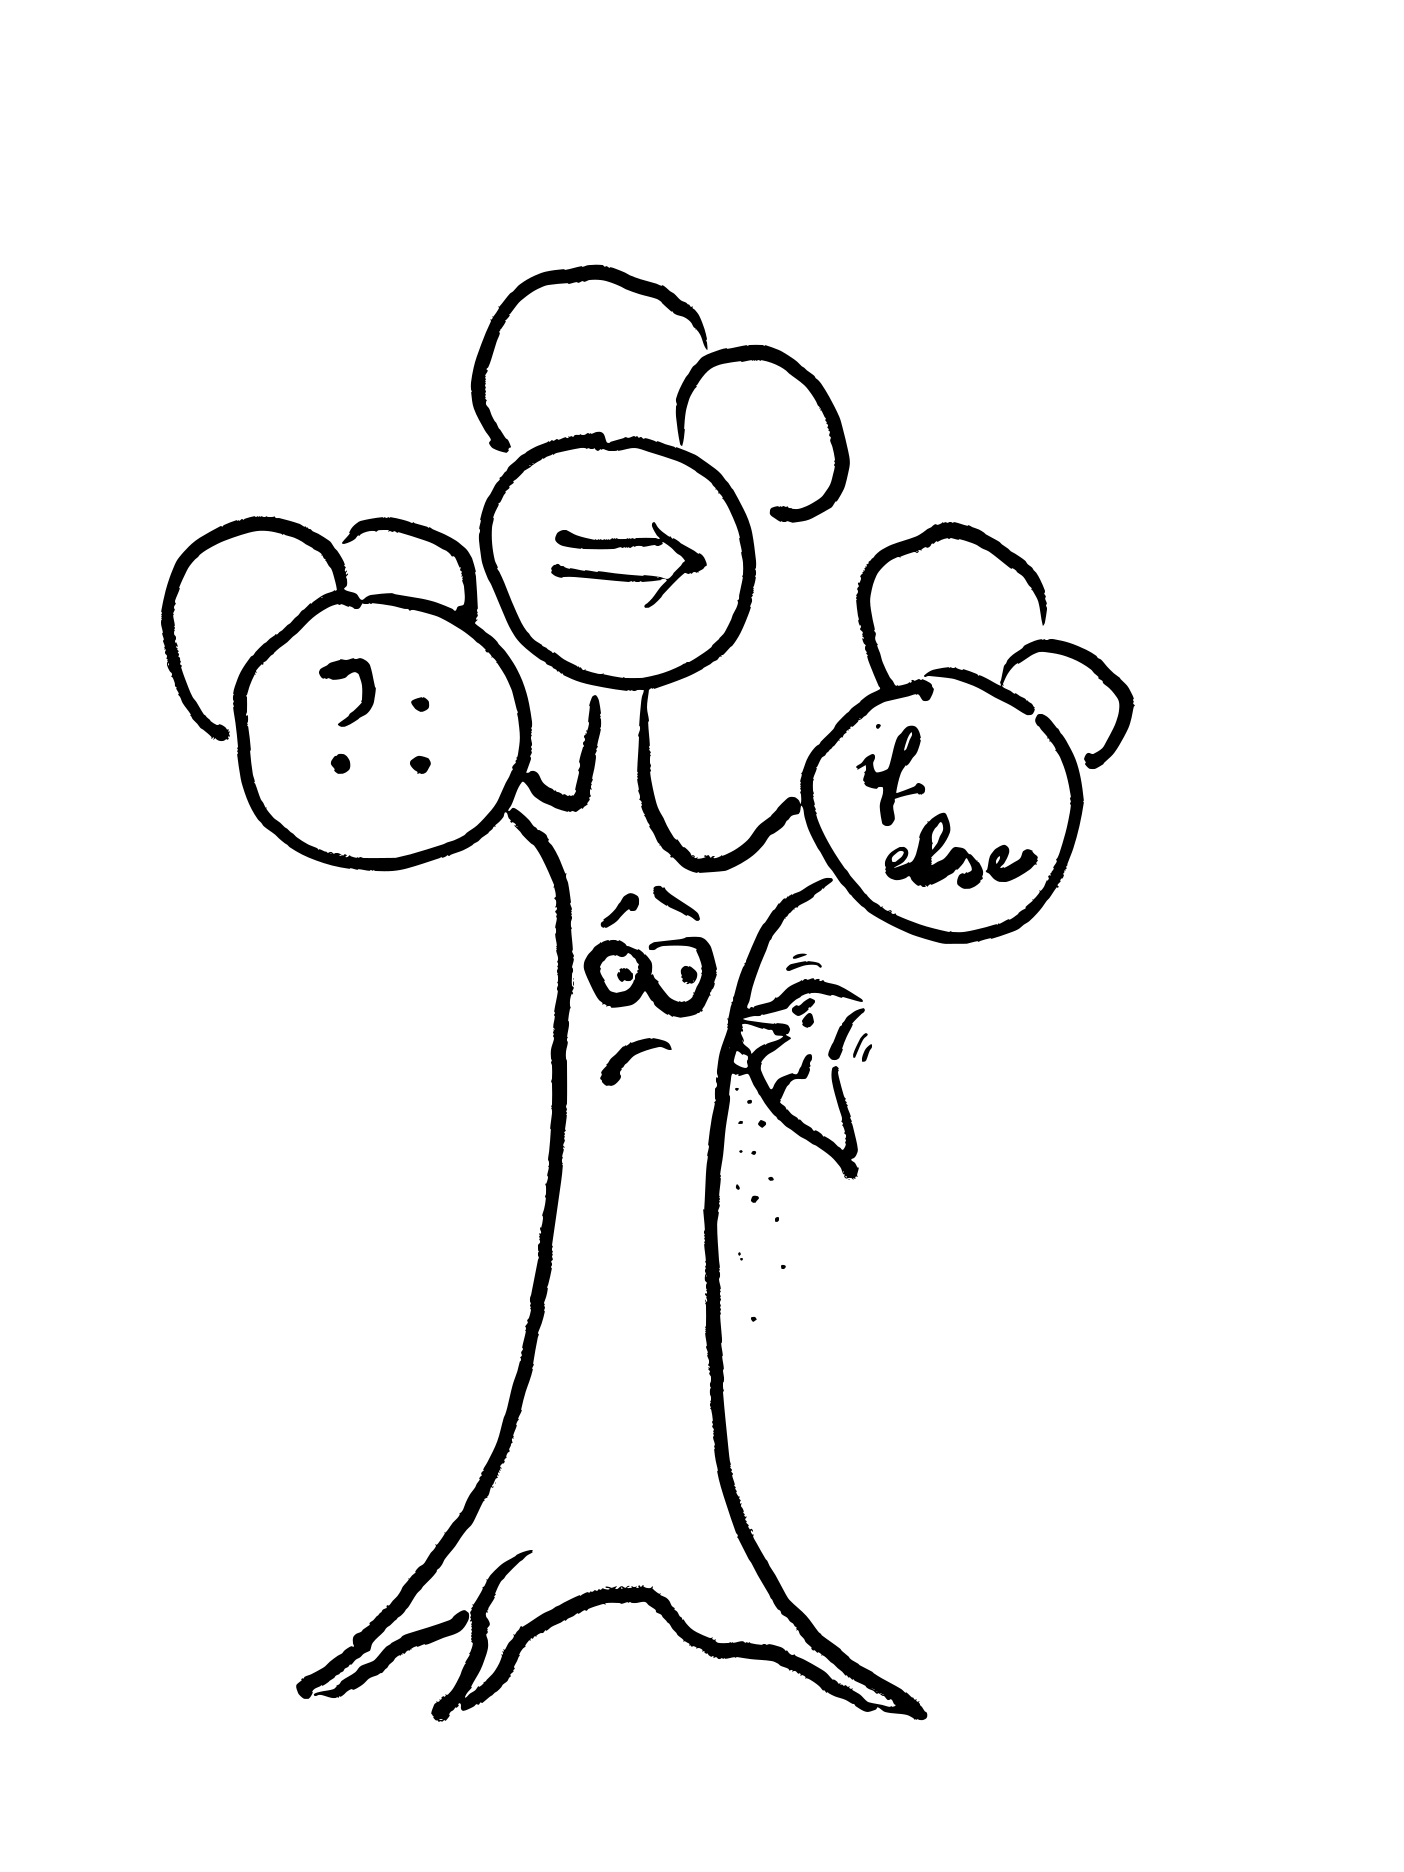
\includegraphics[width=0.9\textwidth]{tree}
    \end{center}

    \newpage
    \section{Approach} \label{p2-approach}

    \subsection{Where to Join} \label{where-to-join}

    For verifying a program, Silicon symbolically executes the program,
    and a symbolic state keeps track of all possible program states at the current point of execution, for all
    possible input values of the program. When encountering certain expressions or statements, for example an
    if-statement, symbolic execution branches into two execution paths, where in
    one path the if-statement is assumed to evaluate to true, and in the second path to false.
    In the following sections, we list the different statements and expressions 
    that result in a branching of execution paths, which later can be joined again.
    
    \begin{lstlisting}[language=Scala, caption={An example Viper program to demonstrate how branching relates to the number of symbolic execution paths. Let \texttt{s0}, \texttt{s1}, \texttt{s2} and \texttt{s3} denote generic viper statements.}, label={lst:viper-branching-example}]
method test(b: Bool) {
    s0
    if (b) {
        s1
    } else {
        s2
    }
    s3
}       
    \end{lstlisting}

    \begin{figure}[H]
        \begin{center}
            \includegraphics[width=0.4\linewidth]{example-execution-paths.png}
            \caption{
                The symbolic execution paths taken by Silicon
                when verifying the program in listing \ref{lst:viper-branching-example}.
                Note that \texttt{s3} is symbolically executed twice as
                the paths are not joined after the if-statement.
            }
            \label{fig:example-execution-paths}
        \end{center}   
    \end{figure}

    \subsubsection{If-Statements} \label{if-statements}

    Viper is parsed into a control flow graph (CFG) consisting of blocks containing
    statements, and edges that connect blocks. Edges can be unconditional or conditional,
    and can potentially form cycles whenever a back edge is connected to a loop head block.
    Silicon branches whenever a block has more than one outgoing edges.
    To join again at the correct location within the CFG after branching,
    the join point for each corresponding branch point has to be identified.
    The algorithm used to identify join points within the CFG is discussed later in
    \ref{finding-join-points}

    \subsubsection{Conditional Expressions}

    Consider a conditional expression of the form \texttt{$b$ ? $e_1$ : $e_2$}.
    As Silicon evaluates this expression, and $b$ cannot definitely be evaluated to true or false,
    two branches are created, in the first one, $b$ is assumed to be
    true, and the expression is evaluated to be $e_1$.
    In the second branch, $b$ is assumed to be false, and the evaluation yields $e_2$.
    The symbolic execution is continued in both branches, and all following code
    is executed twice.


    \subsubsection{Implications}

    Similar to conditional expressions, symbolic execution branches on implications too. Consider
    an implication of the form \texttt{$b_1$ ==> $b_2$}. Again, in the first branch, $b_1$ is assumed to be true,
    and in the second branch, $b_1$ is assumed false.

    \subsection{Pros and Cons of Joining}

    Branches created by conditional expressions and implications are already being joined if they are pure,
    that is, they do not modify the heap.
    Branches resulting from impure conditional expressions and implications,
    and from all if-statements aren't joined again, meaning that
    all statements later down the verification path are evaluated twice, as demonstrated
    in the example of figure \ref{fig:example-execution-paths}. Both of these
    verification paths may branch again, eventually leading to exponential growth in branches.
    These branches are avoided when joining the symbolic execution paths back together.

    Intuitively, the same work has to be done with or without joining, but 
    there are some differences
    when joining. Concretely, joining leads to
    fewer execution paths but with more complex symbolic states.
    Table \ref{joining-comparison} lists some differences.

    \begin{center}
        \begin{tabular}{ l|l|l }
            Property & Without Joining & With Joining \\
            \hline
            Number of Execution Paths & More Paths & Fewer Paths \\
            Symbolic State & Less Complex & More Complex \\
            Number of SMT Solver Invocations & More Invocations & Fewer Invocations \\
            Complexity of SMT Solver Invocations & More Complex & Less Complex
        \end{tabular}
        \captionof{table}{Differences of using symbolic execution with joining versus without joining.}
        \label{joining-comparison}
    \end{center}


    \subsection{Merging the Symbolic State} \label{merging-the-symbolic-state}
    
    After finding the appropriate locations for joining, the information
    gathered through both branches in the symbolic state has to be merged
    into a single symbolic state to continue the symbolic execution on a single
    path.

    To formalize the merging process, we define
    a symbolic state $\sigma$ of type $\Sigma := (\Gamma, \Pi, H)$. The entries
    defined as follows:

    \begin{itemize}
        \item A store $\gamma$ of type $\Gamma := Var \to V$ maps local variables to their symbolic values.
        \item A path condition stack $\pi$ of type $\Pi$ records all assumptions that have been made on the current verification path.
        \item A symbolic heap $h$ of type $H$ that records which heap locations are accessible and their respective symbolic values.
            A heap is implemented as a collection of heap chunks, where each heap chunk provides information
            about the location's value and the receiver's permission amount to the location.
    \end{itemize}

    For the following subsections, assume that after the verification branched under the condition $c$ of type $Bool$,
    two symbolic states $\sigma_1 = (\gamma_1, \pi_1, h_1)$ under the branch condition $c_1$, and
    $\sigma_2 = (\gamma_2, \pi_2, h_2)$ under the branch condition $c_2$, which is the negation
    of $c_1$, are to be merged,
    resulting in the new state $\sigma_3 = (\gamma_3, \pi_3, h_3)$.

    Note that this core idea could be extended to merge more than two states at once. In 
    the current version of Viper however,
    no more than two states are merged at once.

    \subsubsection{Merging Stores}

    For merging stores $\gamma_1$ and $\gamma_2$, we consider two cases:

    \begin{enumerate}
        \item Let $x \mapsto v$ denote that the variable $x$ maps to the value $v$.
            Assume that for some local variable $x$, we have $x \mapsto v_1 \in \gamma_1$ and $x \mapsto v_2 \notin \gamma_2$.
            In this case, we can simply omit $x$ in the new store $\gamma_3$ as we can assume that $x$ won't
            be needed later down the verification path as Viper has the usual lexical
            variable scopes.
        \item For some local variable $x$, we have $x \mapsto v_1 \in \gamma_1$ and $x \mapsto v_2 \in \gamma_2$.
            In this case, we modify store entry such that $x \mapsto Ite(c_1, v_1, v_2) \in \gamma_3$,
            where $Ite(b, e_1, e_2)$ is a conditional expression that resolves to $e_1$ if $b$ is true, and $e_2$ otherwise.
    \end{enumerate}

    \subsubsection{Merging Heaps} \label{merging-the-heap}

    To merge heaps $h_1$ and $h_2$, we perform the following steps:

    \begin{enumerate}
        \item Every heap chunk $c$ for which $c \in h_1$ and $c \in h_2$ holds can be carried over to $h_3$
            without modifications.
        \item Let $r.f \mapsto v \perm p$ denote a heap chunk where $r$, $v$, $p$ are symbolic expressions
            denoting the receiver of some location $f$, the symbolic value of the location and the permission
            amount provided by the heap chunk.
            Heap chunks $ch := r.f \mapsto t \perm p$ where $ch \in h_1$ and $ch \notin h_2$ are modified to
            have permissions only if $c_1$ holds: $ch' := r.f \mapsto v \perm Ite(c_1, p, 0) \in h_3$.
    \end{enumerate}

    Quantified heap chunks are of the shape
    $\forall r: r.f \mapsto v(r) \perm p(r)$.
    Analogously to non-quantified heap chunks described previously,
    we can simply modify the permission amounts of
    quantified heap chunks to $p'(x) = Ite(c_1, p(x), 0)$.
    
    %Note that our heap merging implementation may
    %introduce multiple heap chunks for the same location due to fractional permissions.
    %Silicon provides a mechanism called state consolidation
    %that can be used to avoid this issue.
    %but doing a state consolidation
    %after every merge has shown to decrease performance.
    %Instead, we avoid state consolidation after each merge all together.

    Proving assertions or permission amounts of a location in the heap
    is normally done greedily, where the heap chunks are
    traversed until the first matching heap chunk for the location is found.
    This greedy algorithm is in general incomplete if multiple heap chunks for the same location
    exist. To avoid any issues,
    Silicon's option \texttt{--enableMoreCompleteExhale} should be used,
    which enables a more sophisticated method of finding matching heap chunks.
    Furthermore, more complete exhale provides a small performance improvement
    by itself, as later discussed in section \ref{more-complete-exhale}.

    Another option to avoid incompleteness is to do state consolidations
    after merging heaps. State consolidations can rewrite the heap using the information
    available in the current state such that aliasing heap chunks can be combined into a single one.
    Doing state consolidations after every merge has shown to decrease performance, which is why
    we require more complete exhale to be enabled instead.

    %Quantified heap chunks are of the shape $\forall x: c(x) \implies e(x).f \mapsto v(x) \perm p(x)$.
    %In practice, they are rewritten to the equivalent form $\forall x: e(x).f \mapsto v(x) \perm p'(x)$,
    %where $p'(x)$ is defined as:

    %\begin{math}
    %    p'(x) = \begin{cases}
    %        p(x) & \text{if } c(x) \text{ is true,} \\
    %        0 & \text{else}
    %    \end{cases}
    %\end{math}

    \subsubsection{Merging Path Conditions}

    For path conditions, the functionality for merging is already provided.
    This is done by putting the collected path conditions of each branch
    under an implication with the corresponding branch condition.


    \subsubsection{An Example}

    Assume we want to merge two following two symbolic states:
    
    \begin{math}
        \sigma_1 = (\{a \mapsto 7\}, \{b <= 10\}, \{x.f \mapsto 7 \perm 1\}) \text{ with branch condition } b <= 10 \\
        \sigma_2 = (\{a \mapsto 8\}, \{b > 10\}, \{y.f \mapsto 8 \perm 1\}) \text{ with branch condition } b > 10
    \end{math}

    As $a$ occurs in the store of both $\sigma_1$ and $\sigma_2$,
    the new store entry has the shape $a \mapsto Ite(b <= 10, 7, 8)$.

    For the heap, we cannot be sure whether the receivers $x$ and $y$
    are aliases, which is why we keep both heap chunks but with modified
    permission amounts: $x.f \mapsto 7 \perm Ite(b <= 10, 1, 0)$, $y.f \mapsto 8 \perm Ite(b > 10, 1, 0)$.

    Finally, the path conditions $b <= 10$, $b > 10$ are merged, resulting
    in a new, empty path condition.

    The new state is now fully described as follows: 

    \begin{math}
        \sigma_3 = (\{x \mapsto Ite(b <= 10, 7, 8)\}, \{\}, \{x.f \mapsto 7 \perm Ite(b <= 10, 1, 0), y.f \mapsto 8 \perm Ite(b > 10, 1, 0)\})
    \end{math}

    \newpage
    \section{Implementation}

    \subsection{Finding Join Points} \label{finding-join-points}

    In section \ref{where-to-join}, we have discussed which statements and expressions cause
    branches that can be joined again, but we still need to identify the join points.
    For conditional expressions and implications, finding the join point is trivial
    as it is within the same expression as the branch point.
    For if-statements, finding the join point to a corresponding branch point is more 
    difficult as we have to search
    for if within the whole CFG.
    We introduce a recursive algorithm which maps each branch point to its corresponding join point,
    if it exists. The algorithm runs the following steps:

    \begin{enumerate}
        \item Initialize a queue of blocks to visit next (the successors of the branch point),
            and a list of already visited blocks (the branch point itself).
            Traverse the CFG in a breath-first way by adding the successors of a block
            to the queue (listing \ref{lst:join-point-algorithm}, line 9).
        \item \emph{Base Case.} If a block is visited that already is included in the visited list,
            return this block (listing \ref{lst:join-point-algorithm}, line 16), as it is the join point corresponding to the branch point where this algorithm was called.
        \item \emph{Recursive Case.} If a block has two outgoing edges, it is a branch point.
            Call this algorithm recursively, starting from this branch point (listing \ref{lst:join-point-algorithm}, line 13).
    \end{enumerate}

    \begin{lstlisting}[language=Scala, caption={The join point finding algorithm without support for loops.}, label={lst:join-point-algorithm}]
def findJoinPoint(branchPoint: CFGNode)
    queue = branchPoint.successors
    visited = [branchPoint]
    // Abort while the loop if no next node is given.
    while curr = queue.next
        if curr not in visited
            visited += curr
            match curr.successors
                case [next]:
                    queue += next
                // Branch point found,
                // find corresponding join point recursively.
                case [_, _]:
                    queue += findJoinPoint(curr)
                // Currently, only CFGs with at most two outgoing
                // edges are considered.
                case _:
                    abort("At most two outgoing edges are supported")

        else
            // curr is the join point for this branch point.
            return curr

    
        
    \end{lstlisting}

    Special attention has to be paid to loops. If our algorithm follows a back edge before finding a join point,
    it may do the recursion again for the same branch point, leading to non-termination.
    Figure \ref{fig:join-point-problem} shows an example CFG where this problem occurs.
    To avoid this issue, all already visited loop head blocks (they are already labeled as such)
    are remembered for later recursive invocations. Already visited loop head blocks are not followed again.
    
    \begin{figure}[H]
        \begin{center}
            \includegraphics[width=0.6\linewidth]{join-point-problem.png}
            \caption{
                An example where the naive join point finding algorithm sketched in 
                listing \ref{lst:join-point-algorithm}
                fails. Starting at the branch point, the edges are visited in a breath-first way, as indicated by
                the numbers. Due to the loop, the initial branch point is found again before finding
                the join point, and the same recursion is done again.
            }
            \label{fig:join-point-problem}
        \end{center}   
    \end{figure}

    To find join points within the CFG, the algorithm described in listing \ref{lst:join-point-algorithm} is implemented,
    but with some additional modifications to support loops. All loop heads that
    were already seen are remembered to avoid infinite recursion issues as described
    in figure \ref{fig:join-point-problem}.
    In a single preprocessing step, the algorithm produces a mapping from each branch point to the respective join point.
    If an if-statement is encountered during verification, we check if a 
    corresponding join point exists and the branches can be joined again.
    Otherwise, we branch as normal without joining again.

    \subsection{Implementing State Merges} \label{implementing-state-merges}

    Store and heap merges are implemented as according to section \ref{merging-the-symbolic-state}.
    Silicon's state, however, consists of additional data, that has to be merged with caution.
    Some of these additional state components are used at various times during verification
    to increase performance.
    Such caches within the state are currently emptied instead of merged for simplicity.
    Furthermore, the option
    \texttt{--disableCaches}, which disables the caches,
    was added to Silicon in order to provide more fair benchmarks.
    The performance impact of disabling caches is further discussed in section \ref{disable-caching}.

    Our implementation can be optionally enabled by passing the command-line
    argument \texttt{--moreJoins} to the Silicon executable. To illustrate the difference
    in verification, consider the Viper program in listing \ref{lst:viper-example}.
    Table \ref{execution-1} shows the execution trace of Silicon with more joins disabled,
    in table \ref{execution-2}, more joins is enabled.

    \begin{lstlisting}[language=Scala, caption={An example Viper program.}, label={lst:viper-example}]
method test(b: Bool) {
    var x: Int := 0
    if (b) {
        x := x + 5
    } else {
        x := x + 7
    }
    x := x + 3
    assert x <= 10
}       
    \end{lstlisting}

    \begin{center}
        \begin{tabular}{ l|l|l|l }
            Line (Listing \ref{lst:viper-example}) & Operation & Store & Path Conditions \\
            \hline
            2 & \texttt{var x: Int := 0} & & \\
            4 & \texttt{x := x + 5} & $x \mapsto 0$ & $b$ \\
            8 & \texttt{x := x + 3} & $x \mapsto 5$ & $b$ \\
            9 & \texttt{assert x <= 10} & $x \mapsto 8$ & $b$ \\
            6 & \texttt{x := x + 7} & $x \mapsto 0$ & $!b$ \\
            8 & \texttt{x := x + 3} & $x \mapsto 7$ & $!b$ \\
            9 & \texttt{assert x <= 10} & $x \mapsto 10$ & $!b$ \\
        \end{tabular}
        \captionof{table}{Symbolic execution trace of viper program \ref{lst:viper-example} using the base implementation without joining.}
        \label{execution-1}
    \end{center}

    \begin{center}
        \begin{tabular}{ l|l|l|l }
            Line (Listing \ref{lst:viper-example}) & Operation & Store & Path Conditions \\
            \hline
            2 & \texttt{var x: Int := 0} & & \\
            4 & \texttt{x := x + 5} & $x \mapsto 0$ & $b$ \\
            6 & \texttt{x := x + 7} & $x \mapsto 0$ & $!b$ \\
            8 & \texttt{x := x + 3} & $x \mapsto Ite(b, 5, 7)$ & \\
            9 & \texttt{assert x <= 10} & $x \mapsto Ite(b, 5, 7) + 3$ & \\
        \end{tabular}
        \captionof{table}{
            Symbolic execution trace with joining.
            Joining leads to fewer execution steps,
            but to a more complex state.
        }
        \label{execution-2}
    \end{center}

    \newpage
    \section{Evaluation}

    In the following section \ref{performance-evaluation}, we analyze the performance difference
    of our implementation using more joins, compared to the base implementation,
    which only joins on simple cases, as described in \ref{p2-approach}. Additionally, we provide some complementary benchmark results
    which provide additional insights. 


    \subsection{Performance Evaluation} \label{performance-evaluation}
    
    The benchmark uses frontend-generated Viper programs from VerCors \cite{vercors},
    Prusti \cite{prusti}, Gobra \cite{gobra}, Vyper \cite{vyper} and Nagini \cite{nagini}
    as we are interested in the performance impact on verifying real-life examples, and
    the total duration of each verification run is measured.
    The benchmark is repeated five times, where the
    slowest and fastest verification times are ignored.
    The results show that verification time
    decreases by around 3\% on average when using more joins,
    relative to a version which doesn't
    make use of the implemented joining procedures.
    Intuitively, one would expect that fewer branches lead to better
    performance, however, state merging introduces a more complex final state which again tends to worsen
    performance.
    
    When comparing the number of state merges 
    to the verification time performance difference, no clear correlation is
    visible, as can be seen in figure \ref{fig:state-merges}.

    \begin{figure}[H]
        \includegraphics[width=\linewidth]{state-merges-vs-performance.png}
        \caption{
            Impact on the number of state merges on the performance,
            negative performance difference shows a speedup.
        }
        \label{fig:state-merges}
    \end{figure}

    Interestingly, figure \ref{fig:absolute-verification-time} shows that the performance seems to
    improve for about 3.3\% of the programs
    with an absolute base verification time of up to 0.5 seconds. With increasing verification
    time, the performance decreases, and for programs with a verification time greater
    than 10 seconds, we get a decrease of performance.
    
    This observation suggests that for smaller programs where fewer joins are needed, the more complex symbolic
    states caused by joining is worth trading for the benefit of having fewer branches. For
    larger programs, the symbolic state may become overly complex up to a point that the advantage of
    fewer branches no longer pays off.

    \begin{figure}[H]
        \includegraphics[width=\linewidth]{performance-change-vs-verification-time-part-2-no-warnings-counted.png}
        \caption{
            Change in performance depending on absolute base verification time.
            Negative performance difference shows a speedup.
            Excluded are programs where no joins were performed on verification.
            The numbers in the brackets indicate the number of test cases falling in each section.
        }
        \label{fig:absolute-verification-time}
    \end{figure}

    \subsection{Complementary Benchmarks}

    \subsubsection{Disable Caching} \label{disable-caching}

    As state merging currently empties caches instead of merging them, an
    option to disable the caches entirely was added to Silicon in order to
    provide more fair benchmarks.
    Disabling caches results in a performance decrease of 1.9\%
    compared to the base implementation with caching enabled. In the base implementation used
    for comparison in section \ref{performance-evaluation}, the caches were disabled
    such that the performance of both implementations are not affected by caching.

    \subsubsection{More Complete Exhale} \label{more-complete-exhale}

    Silicon additionally provides an option of enabling a more complete version
    of exhaling permissions, which should be used when joining is enabled,
    as discussed in section \ref{merging-the-heap}.
    Benchmarks have shown that enabling more complete 
    exhale results in a performance increase of 2.9\%. In the benchmark presented
    in section \ref{performance-evaluation}, more complete exhale was used
    by both implementations such that this performance increase observed by using this feature
    does not affect the results.


    \newpage
    \section{Conclusion and Future Work}

    We have presented an approach for joining verification branches
    in Silicon, and discussed the advantages and disadvantages of
    joining. The benchmark has shown that joining does not generally lead
    to a performance improvement when verifying programs.
    Nevertheless, there are still some open questions 
    that can be addressed in future work:

    \begin{itemize}
        \item Currently, we use conditional expressions for merging both
            the heap and the store. Merging can also be done by introducing
            new symbolic variables and conditionalizing them via implications
            in the path conditions. For example, if the store is merged to
            $v = Ite(b, e_1, e_2)$, we could analogously express this using
            a new symbolic variable $v'$ as
            $v = v'$ and restrict the value of $v'$ in the path conditions using implications
            $b \implies v' = e_2$ and $\overline{b} \implies v' = e_2$.
            Maybe, The implementation of merges using
            implications instead of conditional expressions
            will lead to a performance increase.
        \item Section \ref{implementing-state-merges} discusses how caches are
            used in Silicons state. For simplicity, we empty such caches
            instead of merging them. Implementing sophisticated cache merges would
            probably result in a performance increase when using more joins.
        \item The current implementation described in part \ref{part-2}
            has introduced a bug which in a few cases (7 of the 333
            tests used in the benchmark were affected) leads to a failure
            in the interaction with the SMT solver Z3 \cite{z3} that Silicon
            uses internally. Simply put, the merging of some quantified heap
            chunks may result in a Z3 warning because two triggers,
            that for themselves work flawlessly, may result in a new, invalid
            trigger when merged. The exact details or an approach to fix
            this bug are currently unclear and should be further examined.
    \end{itemize}

    \newpage
    %\bibliographystyle{unsrt}
    \printbibliography

    \includepdf[pages=-]{plagiat-eigenstaendigkeitserklaerung-filled.pdf}

\end{document}